% part_A: 원문 1–8쪽 (제목, 초록, I. 서론, II. 에이전트형 SC의 기초) — 그림 1–4, 표 I–VI
\begin{center}
{\Large\bfseries 에이전트형 의미 통신: 개념, 구조, 비전\par}
\vspace{0.3em}
{\normalsize Agentic Semantic Communication: Concepts, Architectures, and Visions\par}
\vspace{0.8em}
{\normalsize Joonho Seon, \textit{Member, IEEE}, Seongwoo Lee, \textit{Member, IEEE}, Soo Hyun Kim, \textit{Member, IEEE},\\
Young Ghyu Sun, \textit{Member, IEEE}, Hyowoon Seo, \textit{Senior Member, IEEE},\\
Mehdi Bennis, \textit{Fellow, IEEE}, Dong In Kim, \textit{Life Fellow, IEEE}, Jin Young Kim, \textit{Senior Member, IEEE}\par}
\end{center}

{\renewcommand{\thefootnote}{}%
\footnotetext{이 연구는 다음의 지원을 받아 수행되었다. 정부(MIST)의 재원으로 한국연구재단(NRF, National Research Foundation of Korea)의 지원을 받은 과제(RS-202523524307), 정보통신기획평가원(IITP)이 관리하는 과학기술정보통신부(MSIT) 대학ICT연구센터(ITRC) 지원 사업(IITP-2026-RS-2023-00258639), 그리고 정부(MSIT)의 재원으로 한국연구재단(NRF)의 지원을 받은 과제(RS-2026-25496925). [옮긴이: 첫 과제의 부처명 ``MIST''는 뒤의 두 과제와 같은 ``MSIT''의 오기로 보이며, 첫 과제 번호 ``RS-202523524307''도 다른 번호 형식(RS-연도-번호)과 달리 하이픈이 하나 빠져 있다. 둘 다 원문대로 두었다.]

Joonho Seon, Seongwoo Lee, Soo Hyun Kim, Young Ghyu Sun, Jin Young Kim은 광운대학교 전자융합공학과 소속이다(Seoul 01897, South Korea; e-mail: \{dimlight13, swoo1467, kimsoogus, yakrkr, jinyoung\}@kw.ac.kr).

Hyowoon Seo와 Dong In Kim은 성균관대학교 전자전기컴퓨터공학과 소속이다(Suwon 16419, South Korea; e-mail: \{hyowoonseo, dongin\}@skku.edu).

Mehdi Bennis는 University of Oulu 정보기술·전기공학부 무선통신센터(Centre for Wireless Communications) 소속이다(90570 Oulu, Finland; e-mail: mehdi.bennis@oulu.fi).}}

\begin{abstract}
6세대(6G, sixth-generation) 응용에서는 수신기가 받은 정보를 바탕으로 과업을 수행해야 하는 경우가 늘고 있다. 그러나 기존 방식은 과업과의 관련성과 무관하게 비트 수준의 복원을 최적화한다. 그 결과 부족한 전송 자원이 과업과 무관한 정보에 쓰일 수 있고, 요구되는 데이터 전송률을 맞추기가 점점 어려워진다. 통신의 목적과 최적화 대상 사이의 이러한 불일치는 의미 통신(SC, semantic communication)으로의 패러다임 전환을 이끌었다. 기존 서베이들이 SC를 다루었지만, 적응성과 추론 능력을 갖춘 자율적 SC 시스템은 아직 충분히 탐구되지 않았다. 이 연구 공백을 메우기 위해 우리는 에이전트형 SC(ASC, Agentic SC)라는 개념을 제시한다. ASC는 통신 시스템 안의 에이전트가 과업과 환경 변화에 따라 동적으로 지각하고(perceive), 계획하고(plan), 추론하고(reason), 자기 교정(self-correct)할 수 있게 하여 자율성(autonomy)을 강조한다. 이 서베이에서는 ASC의 개념적 토대를 세우고, 시스템 수준 통합 정도에 따른 새로운 SC 분류 체계(taxonomy)를 제안한다. 이 분류 체계 안에서 기존 연구를 검토하고, 대표적 기법을 짚으며, 여러 연구 흐름에서 얻은 교훈을 정리한다. 구체적으로, 대규모 언어 모델, 세계 모델(world model), 외부 지식, 오케스트레이션(orchestration), 창발적 통신(emergent communication)에 기반한 에이전트가 어떻게 자율성과 적응성을 얻을 수 있는지 살펴본다. 아울러 ASC 시스템이 대규모로 동작할 수 있게 하는 협력 통신과 조정(coordination) 전략, 엣지 배포(edge deployment) 기법을 조사한다. 더 나아가 ASC의 유망한 응용과 활용 사례를 제시하고, 시스템 구현을 위한 미해결 과제를 밝히며, 향후 연구 방향을 제안한다.
\end{abstract}

\noindent\textbf{색인어}---의미 통신, 추론 과정, 지식 기반 시스템, 다중 에이전트 강화학습.

\section{서론}

\subsection{동기}
통신이 시작된 이래 연구자들은 기기가 사람의 개입 없이 맥락(context)을 이해하고 의도를 전달하는 지능형 에이전트가 되기를 꿈꿔 왔다 [1]. 오늘날 생성형 인공지능(AI, artificial intelligence)과 에이전트형 AI는 기기가 자율적으로 통신하고, 추론하고, 적응하게 함으로써 이 비전을 현실로 만들고 있다 [2]. 이와 나란히 세계 표준화 기구들은 AI에 기반한 통신 프레임워크를 추진하고 있다 [3]. 이런 흐름 속에서 통신 기기는 더 이상 수동적인 송신기가 아니라 지각과 의사결정 능력을 지닌 자율 에이전트로 여겨진다. 그 기원을 이해하기 위해 Shannon 이론으로 돌아가 통신이 어떻게 발전해 왔는지 짚어 보자.

1948년 C.~E.~Shannon은 통신 과정을 설명하는 정보이론의 토대를 세웠다 [4]. 그의 프레임워크에서는 용량이 제한된 잡음 채널로 기호열을 전송하는 문제가 중심이었다. Weaver는 통신 문제를 기술적(technical), 의미적(semantic), 효과(effectiveness)의 세 수준으로 나누어 이 프레임워크를 더 발전시켰다. 이 세 수준은 통신이 기호의 정확성뿐 아니라 전달되는 의미까지 포괄함을 보여 준다 [1]. 그러나 이후의 연구는 주로 비트 수준의 신뢰도를 높이는 데 집중했다. 6세대(6G) 무선 통신이 등장하면서 통신의 목표는 더 높은 데이터 전송률을 얻는 것에서, 전송된 정보가 과업 성능에 기여하도록 하는 것으로 옮겨 갔다.

비트 단위 효율에서 의미 효율로의 이 전환이 SC 개발의 동기가 되었다. 초기 SC 시스템은 주로 오토인코더(autoencoder) 기반 구조를 썼으며, 비트 단위 복원보다 의미 표현을 전송하는 데 초점을 맞추었다 [5]--[9]. 원시 데이터 입력은 잠재 표현으로 압축되어 전송되고, 이어서 수신기에서 복원된다. 그러나 이러한 시스템은 학습 중에 관찰한 통계적 패턴을 재현하는 데 그친다 [10].

연구자들은 송신기와 수신기가 공유하는 지식 베이스(KB, knowledge base)를 활용해 이 문제를 풀고자 했다 [11], [12]. 그러나 실제 통신 시스템에서는 사용자마다 공유 지식의 범위가 달라 의미적 모호성이 생길 수 있다. 또한 KB를 공유하더라도 송신기의 상황 맥락이 그래프에 부호화되어 있지 않으면 의미적 모호성이 생긴다. 이러한 의미적 모호성은 인지적 추론 과정으로 해소할 수 있다. 이 관점은 빠른 휴리스틱 추론(시스템 1, System 1)과 느린 숙고적 추론(시스템 2, System 2)을 구분하는 인지의 이중 과정 이론(dual-process theory)과 일치한다 [13], [14].

추론은 에이전트가 메시지를 해석하게 해 주지만, 그 해석에 따라 행동하게 해 주지는 않는다. 이 간극을 메우려면 에이전트형 적응이 필요하다. 즉 송수신기가 의미를 수동적으로 전달하는 존재에서 자율적으로 의사결정하는 에이전트로 바뀌어야 한다. 따라서 메시지는 더 이상 단순히 복원되는 것이 아니라, 상호작용을 거치며 맥락에 맞게 조정되고, 협상되고, 함께 진화한다. 이 관점에서 자연스럽게 추론과 적응 지능을 특징으로 하는 에이전트형 의미 통신(ASC)이 등장한다.

압축된 의미를 주로 전송하는 기존 SC 시스템과 달리, ASC 시스템은 통신을 에이전트가 특정 맥락 안에서 지각하고, 계획하고, 추론하는 상호작용 과정으로 본다. ASC는 고정된 프로토콜에 의존하지 않고, 동적인 과업과 동작 조건에서 유연한 상호작용을 가능하게 한다. 동작 면에서 ASC는 시스템 1과 시스템 2를 통합해 효율적인 추론(inference)과 맥락을 고려한 추론(reasoning)을 모두 가능하게 한다. 궁극적으로 ASC는 통신을 단순한 데이터 전달을 넘어 의도를 자율적으로 교환하는 에이전트형 과정으로 규정한다.

\setcounter{table}{0}
\begin{table}[htbp]
\centering
\newcommand{\Full}{{\fontspec{Apple Symbols}●}}%
\newcommand{\Half}{{\fontspec{Apple Symbols}◐}}%
\newcommand{\Empt}{{\fontspec{Apple Symbols}○}}%
\caption{ASC의 핵심 주제에 대한 기존 서베이와 이 서베이의 다루는 범위 비교}
\label{tab:1}
\footnotesize
\renewcommand{\arraystretch}{1.2}
\begin{tabularx}{\linewidth}{|c|Y|c|c|c|c|c|}
\hline
\textbf{참고문헌} & \centering\arraybackslash\textbf{기여} & \textbf{\makecell{맥락적\\추론}} & \textbf{\makecell{생성형\\AI}} & \textbf{\makecell{에이전트형\\AI}} & \textbf{\makecell{창발\\언어}} & \textbf{\makecell{다중 에이전트\\시스템}} \\
\hline
[15] & 다중 에이전트 SC를 위한 3계층 SC 네트워크 구조와 보안·프라이버시 분류 체계를 제안한다. & \Half & \Empt & \Half & \Empt & \Full \\
\hline
[16] & 의미를 신선도(freshness) 및 과업 효용과 통합해 효율을 강조하는 Intellicise 패러다임을 제안한다. & \Half & \Half & \Empt & \Empt & \Half \\
\hline
[17] & 현재 데이터 기반 의미 시스템의 한계를 분석하고, 지식 중심 통신으로 옮겨 갈 때의 장점을 부각한다. & \Full & \Empt & \Empt & \Half & \Empt \\
\hline
[18] & 우주-공중-지상-해양 통합 네트워크 전반의 SC를 조사하고, 폐루프(closed-loop) 지각-통신-계산-구동-상호작용 프레임워크를 소개한다. & \Half & \Half & \Empt & \Empt & \Half \\
\hline
[19] & 그래프 신경망, 다중 에이전트 심층 강화학습, 확장 가능한 네트워크 최적화를 위한 심층 강화학습을 포함한 여섯 가지 학습 기반 최적화(learning-to-optimize) 프레임워크를 조사한다. & \Half & \Half & \Empt & \Empt & \Half \\
\hline
[20] & 역사적 관점, 분류 체계, 데이터셋을 하나로 묶어 의미 통신에 대한 포괄적 튜토리얼을 제공한다. & \Full & \Half & \Empt & \Half & \Half \\
\hline
[21] & 무선 네트워킹을 위한 생성형 AI와 그 과제를 조사한다. & \Half & \Full & \Half & \Half & \Half \\
\hline
[22] & SC의 자원·보안·프라이버시 문제를 통합하고 의미 지표를 재정의한다. & \Half & \Half & \Empt & \Empt & \Half \\
\hline
\textbf{이 서베이} & 제안한 분류 체계에 따라 초기 SC부터 ASC까지의 연구를 검토하며, 특히 맥락적 추론, 생성형 AI, 에이전트형 AI, 창발 언어, 다중 에이전트 시스템 등 ASC 관련 연구를 제시한다. & \Full & \Full & \Full & \Full & \Full \\
\hline
\end{tabularx}

\vspace{0.3em}
\small \Full\ : 충분히 다룸 \quad \Half\ : 부분적으로 다룸 \quad \Empt\ : 다루지 않음
\end{table}

\subsection{기여와 범위}
SC 방법에 관한 기존 서베이들은 모델 구조, AI 네이티브(AI-native) 네트워크, 미래 네트워크 프레임워크를 다루었다 [15]--[18]. 딥러닝, KB, 인과 추론(causal inference), 생성형 AI와 관련된 방법이 SC의 핵심 기반 기술로 조사되었다 [15], [18]--[21]. 전통적인 지표를 넘어 성능 평가를 위한 의미 지표와 효과 지표도 논의되었다 [15], [16], [20]. 자원 관리 전략도 폭넓게 논의되었다 [22]. 또한 위협에 맞서는 프라이버시 관련 방어 기법도 검토되었다 [15], [22]. 그러나 표~\ref{tab:1}에 정리했듯이, 기존 서베이에서 ASC의 핵심 주제는 다루어지지 않았거나 부분적으로만 다루어졌다. 특히 맥락적 추론, 생성형 AI, 에이전트형 AI, 창발 언어(emergent language), 다중 에이전트 시스템 같은 ASC의 핵심 요소는 충분히 다루어지지 않았다.

기존 SC에 구조적 제약이 있음을 생각하면 기존 연구의 이러한 공백은 더욱 두드러진다. 근본적으로 기존 SC 모델은 \emph{무엇을} 전송할지에 초점을 맞춘다. 그러나 이 모델들에는 통신이 \emph{왜}, \emph{언제}, \emph{어떻게} 이루어져야 하는지 스스로 판단하는 능력이 없다. 더욱이 송신기와 수신기를 쌍으로 설계하고 공유된 고정 KB에 의존하는 방식은 확장성(scalability)을 제한한다. 예를 들어 [23]을 따르면, 확장성이란 정해진 가중 매개변수 범위 안에서 확장성 매개변수가 커지더라도, 선택한 기준 시스템에 견주어 과업 수행 품질을 유지하는 시스템의 능력이다. 여기서 확장성 매개변수는 종단점(endpoint)의 수이고, 과업 수행 품질은 과업 성공률이다. 의미 부호기-복호기는 쌍과 과업마다 학습되므로, 모든 쌍 연결에 걸쳐 학습하고 동기화해야 하는 모델 수가 $\mathcal{O}(N^2)$으로 늘어난다 [15]. 이렇게 늘어나면 학습, 동기화, 메모리 비용이 커지고 과업 성공률을 유지하는 능력이 제한될 수 있다. 반면 ASC는 에이전트가 \emph{왜}, \emph{언제}, \emph{어떻게} 통신할지를 적응적으로 추론하게 함으로써 통신 패러다임을 재정의한다. 에이전트는 채널과 과업 조건에 맞춰 전략을 조정하고, 예측된 의미 잠재 상태에 따라 전송을 일으키거나 억제한다. 이러한 기능은 세계 모델, 대규모 언어 모델(LLM, large language model), 다중 에이전트 조정으로 뒷받침할 수 있다. 아울러 ASC에서 이들의 기능은 대역폭, 지연, 잡음, 상호운용성을 포함한 통신 제약의 맥락에서 재해석된다.

우리가 아는 한, ASC 관련 연구의 범위, SC와의 차이점과 공통점, 향후 연구 방향을 체계적으로 정리한 서베이 연구는 없다. 이 서베이는 이러한 공백을 메운다. 또한 이 서베이는 ASC를 통신을 개념화하는 방식과 미래 시스템을 설계하는 방식을 재정의하는 패러다임 전환으로 자리매김한다.

\setcounter{figure}{0}
\begin{figure}[htbp]
\centering
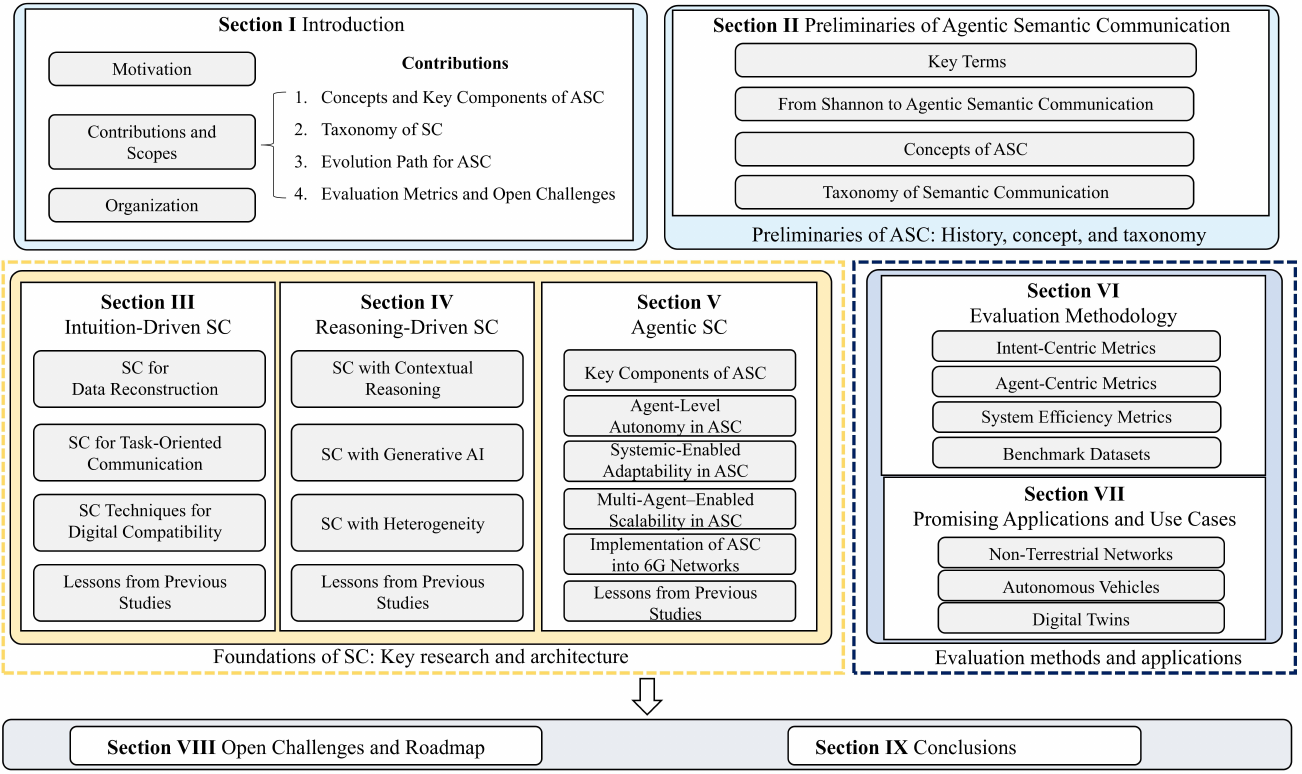
\includegraphics[width=\linewidth]{fig/fig1.png}
\caption{서베이의 구성.}
\label{fig:1}
\end{figure}

이 서베이는 ASC의 지형을 규정하는 세 가지 근본 연구 질문(RQ, research question)을 다룬다.
\begin{enumerate}[label=\arabic*)]
\item \textbf{RQ1 -- ASC의 구조 설계:} 어떤 설계 원칙이 있어야 ASC 시스템에서 에이전트가 맥락을 효율적으로 공유하고, 의미를 협상하고, 자율적으로 결정을 내릴 수 있는가?
\item \textbf{RQ2 -- ASC에서의 학습과 적응:} ASC에서 의미를 파악하고 추론을 수행하는 데, 특히 자율성에 기반할 때, 어떤 학습 전략이 효과적인가?
\item \textbf{RQ3 -- 의도 평가:} ASC 시스템은 의미 정렬과 의도 보존을 어떻게 측정할 수 있는가?
\end{enumerate}

이 세 연구 질문을 다룸으로써 얻은 이 서베이의 기여는 다음과 같이 요약할 수 있다.
\begin{itemize}
\item \emph{ASC의 개념과 핵심 구성 요소} (\textbf{RQ1}): 필수 구성 요소를 통합해 ASC 프레임워크를 개념화한다. 통신 환경에 내재한 제약 안에서 새로운 지능 요소(예: LLM, 세계 모델, KB)가 더해질 때 이 기술들을 어떻게 다시 생각해야 하는지 설명한다.
\item \emph{SC의 분류 체계} (\textbf{RQ1, RQ2}): SC 방식을 추론 능력과 적응성 수준에 따라 분류한다. SC 시스템을 구조나 AI 기법으로 분류한 기존 서베이와 달리, 제안하는 분류 체계는 세 가지 통신 설계 축, 곧 지식의 위치, 의미를 추론하는 과정, 적응적 추론(inference)-추론(reasoning) 제어의 유무를 따라 구성된다.
\item \emph{ASC로의 진화 경로} (\textbf{RQ2}): LLM 기반 추론, 세계 모델, 다중 에이전트 조정이 자원과 채널 제약 아래에서 \emph{무엇을}, \emph{언제}, \emph{어떻게} 통신할지라는 질문에 답하는 통신 인지형(communication-aware) 구성 요소로 어떻게 구현되는지 살펴보고, 이를 통해 ASC의 연구 방향을 제시한다.
\item \emph{평가 지표와 미해결 과제} (\textbf{RQ2, RQ3}): 의도 정렬과 에이전트 상호작용을 중심으로 한 평가 지표를 제시하고 벤치마크를 논의한다. 더 나아가 현재 ASC 연구에서 충분히 다루어지지 않은 미해결 과제를 밝힌다.
\end{itemize}

이 연구는 맥락 지식이 없는 초기 SC 모델부터 추론 능력을 갖춘 ASC까지를 포괄하는 서베이를 제공한다. 핵심 주장은 ASC의 새로움이 개별 AI 모듈 자체가 아니라, 통신을 인식하는 방식으로 이 모듈들을 구현하고 시스템 수준에서 공동 설계하는 데 있다는 것이다. 구체적으로 LLM 기반 추론, 계획, 적응적 상호작용, 협력 추론(cooperative inference)을 포함한 ASC의 핵심 기술을 기술한다. 과업 성공 확률, 지연-보상 절충(trade-off) 같은 에이전트형 평가 지표를 검토하고, 벤치마크 데이터셋을 논의한다. 이 서베이는 비지상 네트워크, 자율주행차, 디지털 트윈(digital twin)을 포함한 유망한 ASC 응용을 살펴보고, 미해결 과제를 개괄하며, 향후 연구를 위한 로드맵을 제시한다.

\subsection{구성}
서베이의 구조는 그림~\ref{fig:1}에 나타냈다. 이 서베이의 나머지 부분은 다음과 같이 구성된다. II절에서는 SC에서 ASC로의 진화를 검토하고 ASC의 핵심 개념과 분류 체계를 소개한다. III절에서는 시스템 1 유형으로 특징지어지는 SC 방법을 포괄적으로 조사한다. IV절에서는 시스템 2 유형을 구현한 SC 연구를 기술한다. V절에서는 ASC의 대표적 방법을 소개한다. ASC의 평가 지표와 벤치마크 데이터셋은 VI절에서 기술한다. ASC의 대표적 응용 시나리오와 활용 사례는 VII절에서 살펴본다. 미해결 과제와 향후 연구 방향은 VIII절에서 제안한다. 맺음말은 IX절에 있다.

\section{에이전트형 SC의 기초}

\setcounter{figure}{1}
\begin{figure}[htbp]
\centering
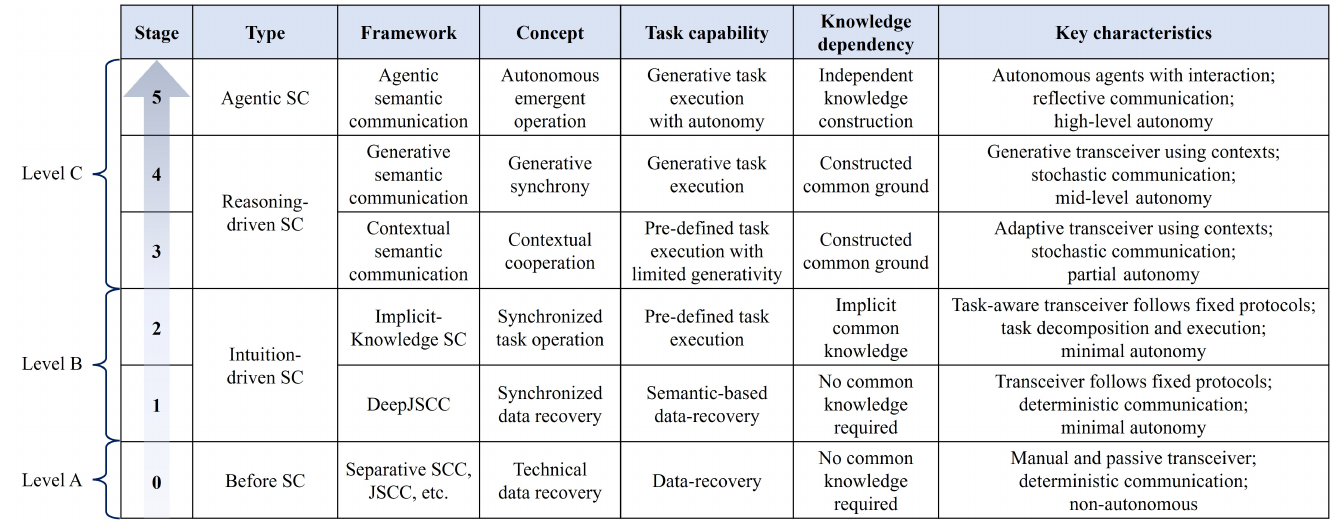
\includegraphics[width=\linewidth]{fig/fig2.png}
\caption{에이전트형 SC로 가는 진화 경로.}
\label{fig:2}
\end{figure}

\setcounter{table}{1}
\begin{table}[htbp]
\centering
\caption{이 글에서 쓰는 핵심 용어}
\label{tab:2}
\small
\renewcommand{\arraystretch}{1.2}
\begin{tabularx}{\linewidth}{|>{\centering\arraybackslash}p{0.2\linewidth}|Y|}
\hline
\textbf{용어} & \centering\arraybackslash\textbf{정의} \\
\hline
\textbf{의도(Intent)} & 송신자가 이루고자 하는 결과로, 전송된 메시지의 기호적 내용 너머에 있다. \\
\hline
\textbf{의미 정렬(Semantic Alignment)} & 상호작용과 추론을 거쳐 메시지의 의미에 대한 공통 이해(공유 맥락)에 이르는 과정과 그 상태. \\
\hline
\textbf{의도 보존(Intent Preservation)} & 의미 정렬이 성공적으로 이루어졌음을 결과 수준에서 보장하는 것. \\
\hline
\textbf{추론(Inference)} & 학습된 모델이 입력이 주어졌을 때 출력을 내는 과정. \\
\hline
\textbf{생성(Generation)} & 학습된 확률 분포에서 표본을 추출해 모델이 새로운 내용을 만들어 내는 추론의 한 형태. \\
\hline
\textbf{추론(Reasoning)} & 모델이 결론에 이르기 전에 중간 논리 단계를 명시적으로 거치는 구조화된 추론 과정으로, 이 글에서는 시스템 2 유형의 처리에 해당한다. \\
\hline
\textbf{사고(Thinking)} & 최종 출력 전까지 중간 단계가 드러나지 않는, 내재화된 형태의 추론. \\
\hline
\textbf{ASC 에이전트(ASC Agent)} & 지각--기억--정책--통신--갱신 루프를 지닌 개체. \\
\hline
\textbf{자율성(Autonomy)} & 외부 지시 없이 자신의 목표를 추구하는 에이전트의 능력. \\
\hline
\end{tabularx}
\end{table}

\subsection{핵심 용어}
이 글 전반에서 쓰는 핵심 용어(예: 의도, 의미 정렬, 의도 보존 등)를 표~\ref{tab:2}에 정리했다.

이 글에서는 \emph{과업 지향}(task-oriented), \emph{의도 기반}(intent-based), \emph{의미 지향(의미적)}(meaning-oriented (semantic)) 통신이라는 용어를 두루 쓴다. 이 용어들은 서로 다른 설계 목표, 최적화 대상, 성공 기준을 가리킨다. 표~\ref{tab:3}은 이들을 구분하고, 이 서베이가 각 단계에서 어떤 개념을 채택하는지 명시한다. III절과 IV절은 의미 지향 설계와 과업 지향 설계를 다루고, V절은 의도 지향(효과 수준) 설계를 다룬다.

\setcounter{table}{2}
\begin{table}[htbp]
\centering
\caption{의미 지향, 과업 지향, 의도 기반 통신의 구분}
\label{tab:3}
\small
\renewcommand{\arraystretch}{1.2}
\begin{tabularx}{\linewidth}{|>{\centering\arraybackslash}p{0.17\linewidth}|>{\centering\arraybackslash}X|>{\centering\arraybackslash}X|>{\centering\arraybackslash}X|}
\hline
\textbf{측면} & \textbf{의미적} & \textbf{과업 지향} & \textbf{의도 기반} \\
\hline
Weaver 수준 & 수준 B & 수준 B--C & 수준 C \\
\hline
전송하는 것 & 원천의 의미를 복구하기 위한 표현 & 알려진 하위(downstream) 과업을 위한 표현 & 의도나 제약을 위한 표현 \\
\hline
최적화 대상 & 원천과 복원 사이의 의미 충실도 & 과업 손실 & 과업 성공과 의도 보존 \\
\hline
설계 단계에서 과업을 아는가? & 반드시 그렇지는 않음 & 예 & 아니요. 추론하거나 협상함 \\
\hline
\end{tabularx}
\end{table}

\subsection{Shannon에서 에이전트형 SC까지}
Shannon--Weaver 모델의 수준 A에서 정보는 메시지의 통계적 불확실성으로 구문적으로(syntactically) 정의되며, 그 발생 확률로 측정된다. 따라서 메시지의 의미적 불확실성은 무시될 수 있다. 예를 들어 수준 A에서는 의미 있는 메시지와 의미 없는 메시지가 같은 양의 정보를 담을 수 있다. 이 경우 의미 오류는 수준 A에서 표현되지 않으므로 바로잡기 어렵다. Shannon은 이 한계를 핵심 과제 가운데 하나로 꼽았으며 [4], Weaver는 통신을 기술적 정확성(수준 A), 의미 해석(수준 B), 행동 효과(수준 C)의 세 수준으로 구성했다 [1].

Shannon--Weaver 모델과 달리, 우리는 이 세 수준을 ASC를 향한 구현 지향 단계로 재구성한다. 그림~\ref{fig:2}는 통신 시스템의 진화를 보여 준다. SC 이전(Before SC)은 수준 A에 해당하는 단계 0이다. 여기서 결정론적 통신(deterministic communication)이란 고정된 프로토콜 아래에서 전송 동작이 미리 정해진 통신을 뜻한다. 단계 1과 2는 기호 복구보다 과업 지향 의미를 우선하며 수준 B를 구현한다. 단계 3, 4, 5는 수준 C에 해당하며, 지식을 통합하고 통신 의도를 정렬한다. SC 이전을 제외하면 통신 유형은 직관 기반 SC, 추론 기반 SC, ASC로 분류된다. SC와 관련된 유형은 분류 체계 소절에서 자세히 다룬다.

6G 비전이 등장하면서 초당 테라비트(Tbps, terabit-per-second) 링크의 필요성과 기계학습(ML, machine learning)의 활용으로 의미 효율이 주목받게 되었다 [16]. 입력 데이터를 단순히 압축한 전송 비트 대신, 수신기가 과업을 수행하는 데 필요한 관련 정보를 전송하는 것이 중요해졌다. 이 요구가 수준 B와 수준 C의 의제를 되살렸고, 이것이 초기 SC의 시작이 되었다 [5].

초기 SC 프레임워크는 송신자와 수신자를 하나의 결합된 심층 오토인코더로 보았다. 초기 SC 모델인 딥러닝 기반 결합 원천-채널 부호화(DeepJSCC, deep learning-based joint source and channel coding) [5]는 단계 1로의 전환을 대표한다. DeepJSCC 모델은 원시 데이터 입력을 저차원 의미 임베딩으로 부호화하고 수신기 쪽에서 이를 복호한다. 그러나 이 방식은 의미 전달보다는 효율적인 데이터 복구에 주로 초점을 맞춘다. 더욱이 공통 지식이 필요 없으므로 지식을 전달하는 능력이 제한된다.

단계 2로서, 이미지 [5]--[7], 음성 [8], 텍스트 [9]의 의미 충실도를 높이는 유망한 해법으로 암묵 지식 SC(implicit-knowledge SC) 방법들이 제안되었다. 수많은 연구가 SC의 초기 개념을 이미지, 음성, 다중 모달 데이터에 적용했다 [6]--[9], [24], [25]. 그러나 초기 SC 연구 대부분은 암묵적 KB와 고정 프로토콜을 갖춘 쌍 설정을 가정했다. 이 가정으로는 에이전트들이 서로 다른 맥락 지식을 지닐 때 생기는 맥락 정렬 문제를 다룰 수 없다. 고수준 통신에서는 송신자와 수신자 사이에 동적인 의미 정렬과 의도 이해가 흔히 요구된다. 수신자가 기호를 복원하더라도 송신자의 의도를 오해할 수 있다.

맥락 불일치를 완화하기 위해 KB가 그래프 형태로 의미 부호기와 복호기에 통합되었다 [11], [12]. 이것이 단계 3에 해당한다. 입력을 그래프의 삼중항(triple)에 대응시킴으로써, 시스템은 과업과 관련된 추론에 필요한 노드에 데이터를 압축한다. KB를 구현하면 의미적 모호성을 줄일 수 있다. 그러나 남은 몇 가지 문제는 충분히 해결하지 못한다. 첫째, KB는 여전히 낡았거나 사용자 사이에 비대칭일 수 있다. 둘째, 상호작용이 일회적(episodic)이어서 오해가 생겼을 때 의미를 협상할 장치가 없다. 마지막으로, 기존 SC 프레임워크는 흔히 쌍으로 된 시스템 1 유형 SC를 가정하므로 [14], 과업이 바뀔 때 적응성이 제한된다.

이러한 간극을 메우려면, 의도한 의미가 정확히 해석되도록 시스템 2의 추론 능력이 필요하다. 맥락 정렬의 부족을 해결하기 위해 추론 능력을 갖춘 SC 방법 [26]이 제안되었다. 대표적 예가 단계 4로 나타낸 생성형 SC(GSC, generative SC)이다. 시스템 1 기반 SC 프레임워크와 달리, GSC에서는 수신기의 생성 과정으로 의미적 모호성을 해소할 수 있다. 수신기에서 원래 의미를 복원하는 대신, 송신자의 맥락을 이용해 의도를 풀어내어(decapsulate) 의미 정렬을 돕는다. 추론 능력이 있음에도, GSC는 생성 모델 고유의 계산 복잡도 때문에 시스템에 부담을 줄 수 있다. 엣지 네트워크처럼 자원과 추론 시간이 제한된 특정 통신 시스템에서는 GSC를 채택하는 것이 실시간 추론에 불리할 수 있다. 따라서 모호한 과업을 효율적으로 수행하려면 시스템 1과 시스템 2의 기능을 모두 수행할 수 있는 향상된 시스템이 필요하다 [13], [14]. 단계(Step) 5에서 기술하는 ASC는 이러한 시스템의 계산 부담을 해결하는 효과적인 해법이 될 수 있다. ASC는 효율적인 추론을 기본으로 쓰고 불확실성이 높거나 분포 밖(OOD, out-of-distribution)인 조건에서만 추론(reasoning)을 호출함으로써, GSC의 지연 비용을 항상 치르지 않고도 강건성을 높일 수 있다. 또한 신경-기호(NeSy, neuro-symbolic) AI는 신경망 기반 특징 추출과 규칙 기반 기호 추론을 결합한다 [27]. 송신자와 수신자가 온톨로지와 추론 규칙 같은 기호 규약을 이미 공유하고 있으면, 고차원 특징 벡터 대신 간결한 기호를 전송할 수 있다. 그러면 메시지당 전송 비용이 줄어드는 대신, 이러한 규약을 미리 배포하고 동기화하는 비용이 든다. ASC 안에서는 에이전트 사이에 KB가 갱신되므로 의미적 모호성을 완화할 수 있다. 전환 기능이 더해지면, GSC의 약점으로 지적된 실시간 추론 면에서도 이점이 생길 것이다.

\subsection{ASC의 개념}
\paragraph{1) 시스템 1과 시스템 2:} 시스템 1과 시스템 2는 의사결정에 대한 상호 보완적인 두 접근을 설명하는 두 개념이다. 시스템 1은 빠르고 직관적이며, 휴리스틱 처리에 의존해 즉각적인 반응을 가능하게 한다. 반면 시스템 2는 더 느리고 신중하게 동작한다. 제안하는 ASC 프레임워크에서는 이 두 개념이 통합된다. 이 이중 시간 척도 동작은 6G 무선 접속 네트워크의 제어 루프와 닮았다. 시스템 1 유형의 추론은 준실시간(near-real-time) 무선 접속 네트워크(RAN, radio access network) 지능형 제어기(RIC, RAN intelligent controller) 루프에, 시스템 2 유형의 추론(reasoning)은 비동기로 동작하는 비실시간(non-real-time) RIC 루프에 대응한다. 표준화된 준실시간(near-RT) RIC 루프는 10~ms--1~s에 걸치지만, 최근의 한 구현은 xApp을 기저대역 장치(baseband unit)와 같은 곳에 배치해 10~ms 미만의 추론을 보고했다 [28]. 이 대응 관계는 V-E절에서 다시 다룬다. 시스템 1, 시스템 2, ASC의 특성은 표~\ref{tab:4}에 종합해 정리했다.

\setcounter{table}{3}
\begin{table}[htbp]
\centering
\caption{시스템 1, 시스템 2, ASC의 특징}
\label{tab:4}
\small
\renewcommand{\arraystretch}{1.2}
\begin{tabularx}{\linewidth}{|>{\centering\arraybackslash}p{0.14\linewidth}|>{\centering\arraybackslash}X|>{\centering\arraybackslash}X|>{\centering\arraybackslash}X|}
\hline
\textbf{특징} & \textbf{시스템 1} & \textbf{시스템 2} & \textbf{ASC (시스템 1과 시스템 2)} \\
\hline
\textbf{인지 과정} & 빠름, 휴리스틱, 직관적 & 더 느림, 논리적, 부담이 큼 & 적응적, 성찰적 \\
\hline
\textbf{핵심 기능} & 패턴 인식, 확률적 추론 & 인과적 추론, 논리적 추론 & 신경-기호 AI, 인지적 성찰 \\
\hline
\textbf{SC에서의 역할} & 효율적인 데이터 복원 & 의미 정렬, 모호성 해소 & 자율적 계획, 맥락 적응 \\
\hline
\end{tabularx}
\end{table}

시스템 1과 시스템 2의 도입은 ML 분야에서 오랫동안 논의되어 온 주제이다. Bengio [29]는 시스템 1 유형 ML에서 시스템 2 유형 ML로 나아가는 연구 방향을 제시했고, Bo Zhang 등 [30]은 시스템 1 유형 ML을 시스템 2 유형 ML에 통합할 것을 주장했다. 이러한 선행 주장에 영향을 받아, 연구자들은 범용 인공지능(AGI, artificial general intelligence)에 이르려면 추론과 패턴 인식을 통합해야 한다는 데 의견을 같이한다. 그 결과 최근 연구는 시스템 1 유형과 시스템 2 유형 ML을 상호 보완적으로 보고 그 통합에 초점을 맞춘다.

이전의 딥러닝 기반 모델 대부분은 방대한 학습 데이터를 활용해 패턴 인식에서 뛰어난 성능을 보였다 [31]. 이러한 모델은 시스템 1 유형 ML 모델로 볼 수 있다. 이 모델들은 인과적 추론 없이 데이터의 통계적 패턴을 내재화하고 확률적 출력을 추론한다. 대표적인 시스템 1 유형 ML 모델인 GPT-4o [32]는 적절한 토큰을 예측하여 적절한 문장을 생성한다. 그러나 경험적 증거에 따르면 논리적 사고가 필요한 과업에서는 환각(hallucination)이 성능을 떨어뜨릴 수 있다 [33]. 시스템 1 유형 ML의 한계를 보완하기 위해 인지적 측면을 반영한 추론 기반 방법론들이 제안되었다 [34]--[36].

최근에는 시스템 1 유형과 시스템 2 유형 ML의 장점을 결합하는 연구가 제안되었다 [27], [37]. 의사결정에 대한 이중 시스템 접근에 기반해 Talker-Reasoner 구조가 제안되었다 [37]. 지연이 짧은 Talker(시스템 1)가 간단한 질의를 처리하고, 불확실성이 높은 사례를 처리할 때는 Reasoner(시스템 2)를 호출한다. NeSy AI를 이용한 또 다른 통합 접근도 제안되었다 [27]. 이 프레임워크에서 에이전트는 인지적 성찰(cognitive reflection)이라는 개념으로 효율과 효과 사이의 균형을 맞출 수 있다. 인지적 성찰이란 자신의 처음 직관적 반응을 점검하고 추론을 거쳐 의도적으로 수정하는 메타인지 과정을 말한다 [27]. 에이전트는 직관적(시스템 1) 답이 기호적(시스템 2) 지식과 모순될 때마다 인지적 성찰을 이용해 그 답을 자동으로 바로잡는다.

\setcounter{figure}{2}
\begin{figure}[htbp]
\centering
\begin{minipage}{0.8\linewidth}\centering
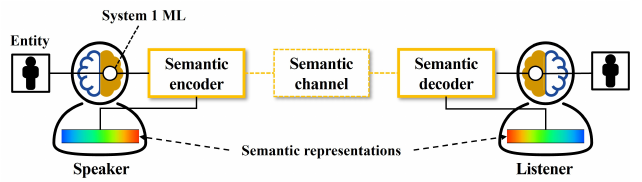
\includegraphics[width=\linewidth]{fig/fig3a.png}\\[0.2em]
{\small (a) 시스템 1 유형 ML을 쓰는 SC}
\end{minipage}\par\vspace{0.8em}
\begin{minipage}{0.8\linewidth}\centering
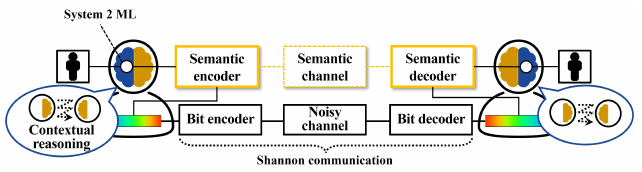
\includegraphics[width=\linewidth]{fig/fig3b.png}\\[0.2em]
{\small (b) 시스템 2 유형 ML을 쓰는 SC}
\end{minipage}\par\vspace{0.8em}
\begin{minipage}{0.8\linewidth}\centering
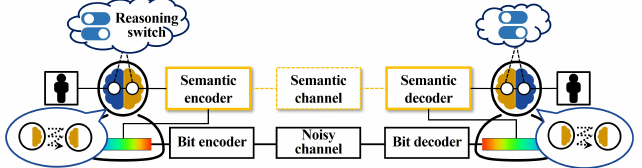
\includegraphics[width=\linewidth]{fig/fig3c.png}\\[0.2em]
{\small (c) 시스템 1 유형과 2 유형 ML을 통합한 SC}
\end{minipage}
\caption{(a) 시스템 1 유형 ML을 쓰는 SC, (b) 시스템 2 유형 ML을 쓰는 SC, (c) 시스템 1 유형과 2 유형 ML을 통합한 SC의 개념도. [13]의 그림을 수정한 것이다.}
\label{fig:3}
\end{figure}

시스템 2 유형 ML에 대한 관심은 커졌지만, SC에 대한 적용은 제한적이었다. SC 프레임워크는 시스템 2 유형 ML 대신, 빠른 추론에 최적화된 시스템 1 유형 ML에 주로 의존해 왔다. Seo [13], Bennis [14], Walid [38]의 연구처럼 최근의 이론적 시도들이 SC의 추론 능력을 논의했지만, 이들은 개념적 측면에 초점을 맞추었다. SC 시스템에 추론 능력을 부여하기 위해 생성형 AI(GAI, generative AI)를 통합하는 접근 [39]이 제안되었다. 그러나 GAI 추론을 계속 호출하면 상당한 지연이 생길 수 있다. 딥러닝 응용과 달리, 대부분의 통신 시스템에서는 추론 지연이 심각한 문제가 될 수 있다. 이 문제를 해결하려면 그림~\ref{fig:3}(c)처럼 SC 프레임워크에 이중 경로 추론 구조를 도입해야 한다.

\paragraph{2) 창발 언어:} 창발 언어(EmLang)는 미리 정의된 프로그래밍 없이 에이전트들의 상호작용에서 자연스럽게 생겨나는 통신 메커니즘을 말한다 [40]. 사람이 설계하는 하향식 패러다임과 달리, EmLang은 통신 프로토콜이 상호작용으로부터 적응적으로 진화하는 상향식 패러다임을 따른다 [41]. EmLang에서는 에이전트들이 주어진 환경 안에서 협력 과업을 풀며, 그 결과로 기호 구조가 발달한다.

ASC는 EmLang의 개념을 받아들여, 에이전트가 통신 행동을 계속 조정하는 상호작용 학습 환경을 가정한다. 이 맥락에서 ASC는 다중 에이전트 강화학습(MARL, multi-agent reinforcement learning)이나 부분 관측 마르코프 결정 과정(POMDP, partially observable Markov decision process) 설정으로 볼 수 있다. 이러한 환경에서 에이전트들은 상호작용하며 메시지를 반복적으로 교환한다. 처음에는 에이전트 사이에 오가는 토큰이 무작위 기호로 이루어진다. 이후 에이전트들은 전송된 기호, 환경 상태, 자기 행동의 결과 사이의 연관을 거듭 찾아낸다. 반복된 상호작용을 거쳐 에이전트들은 의미 있는 표현을 형성하고, 이 표현은 협력 효용을 최적화하는 기호로 수렴한다.

\paragraph{3) 에이전트형 AI, 체화 AI, ASC:} AI 분야에서는 단일 과업 모델을 넘어서는 에이전트를 만드는 데 초점을 둔 새로운 패러다임이 등장했다. 이 에이전트들은 목표를 세우고 과업을 실행할 수 있다. 에이전트형 AI(Agentic AI)라 불리는 이 새로운 패러다임은 불확실하고 동적인 환경에서 목표를 이루기 위한 자율적 지각, 계획, 행동, 학습을 특징으로 한다.

에이전트형 AI와 비슷하지만 구별되는 개념으로 체화 AI(Embodied AI)가 있다. 둘 다 환경과의 상호작용으로 정책을 학습하지만, 체화 AI는 지각과 행동을 완전히 통합된 과정으로 본다. 예를 들어 탁자 위의 사과를 집어 드는 목표를 지닌 로봇이 있다고 하자. 체화 AI에서는 시각 입력과 모터 명령이 되먹임 루프 안에서 동시에 갱신된다. 이 방식은 대개 연속적인 상태 공간과 행동 공간을 지니며, 에이전트는 물리 환경과 상호작용하며 최적 정책을 학습한다. 또한 최근의 체화 AI는 세계 모델을 환경에 대한 사전 지식으로 활용해 미래의 환경 상태를 예측하고 의사결정을 이끈다 [42].

\setcounter{table}{4}
\begin{table}[htbp]
\centering
\caption{체화 AI, 에이전트형 AI, ASC의 특징}
\label{tab:5}
\small
\renewcommand{\arraystretch}{1.2}
\begin{tabularx}{\linewidth}{|>{\centering\arraybackslash}p{0.14\linewidth}|>{\centering\arraybackslash}X|>{\centering\arraybackslash}X|>{\centering\arraybackslash}X|}
\hline
\textbf{특징} & \textbf{에이전트형 AI} & \textbf{체화 AI} & \textbf{에이전트형 SC} \\
\hline
\textbf{범위} & 제어 시스템, 문제 해결 & 로봇공학, 감각운동 과업 & 통신 중심 과업 \\
\hline
\textbf{핵심 기능} & 지각, 계획, 행동, 학습 & 지각과 행동의 결합 & 의미 추출, 계획, 상호작용, 적응 \\
\hline
\textbf{목표} & 목표를 위한 적응적 의사결정 & 물리적 상호작용을 통한 최적 정책 & 의미 충실도, 통신 효율 \\
\hline
\textbf{지식 활용} & 장기 기억, 광범위한 추론 & 물리적 사전 지식 & 중간 수준 기억, 적응적 추론 \\
\hline
\end{tabularx}
\end{table}

ASC는 에이전트형 AI의 일부 원리를 물려받은, 통신 중심 과업의 전문가로 볼 수 있다. 두 시스템은 핵심 속성을 공유하지만 관점은 조금 다르다. 예를 들어 에이전트형 AI는 자율주행, 로봇 제어, 네트워크 관리를 포함한 넓은 영역에서 지각, 계획, 행동, 학습을 다루는 데 쓰여 왔다 [2]. 반면 ASC 시스템은 의미 프로토콜 안에서의 계획, 상호작용, 적응적 동작으로 초점을 좁히며, 지각은 과업 지향 의미 추출로 한정한다. 또한 에이전트형 AI는 장기 기억과 광범위한 추론으로 효과적인 의사결정을 목표로 하는 반면, ASC는 효율적인 통신을 위해 중간 수준 기억(moderate memory)과 적응적 추론을 쓴다. 여기서 장기 기억은 세션을 넘어 유지될 수 있다는 점에서, 에이전트 사이에 공유되는 구조화된 지식을 담은 KB와 구별된다. 반면 중간 수준 기억은 최근의 의미 표현을 수 초에서 수 분 동안 유지하는, 세션 범위의 의미 기억이다. 세 시스템 모두 목표 지향적 행동을 보이지만, 동작 환경의 성격, 행동의 양식, 추론의 범위에서 다르다. 에이전트형 AI, 체화 AI, ASC의 차이는 표~\ref{tab:5}에 요약했다.

\setcounter{figure}{3}
\begin{figure}[htbp]
\centering
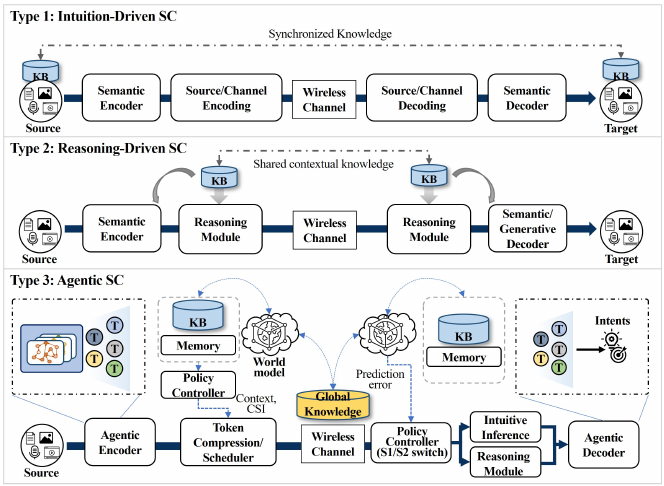
\includegraphics[width=0.85\linewidth]{fig/fig4.png}
\caption{제안하는 의미 통신 시스템 분류 체계의 대표 구조.}
\label{fig:4}
\end{figure}

\subsection{의미 통신의 분류 체계}
앞에서 논의한 시스템 1/2, 명시적 지식, 에이전트형 제어를 바탕으로, 이 소절에서는 SC 시스템의 분류 체계를 소개한다. 기존 SC 분류 체계는 주로 응용 영역 관점(예: 과업 지향 대 데이터 복원), 입력 모달리티, 외부 지식 활용과 자원 제약에 따라 분류한다 [16], [20], [22]. 이러한 관점으로는 시스템이 변화하는 환경에서 어떻게 추론하고 적응하는지를 충분히 설명하지 못한다. 암묵적 추론에서 명시적 추론과 적응적 오케스트레이션으로의 전환에 착안하고 이중 과정 인지에서 영감을 받아, 우리는 SC 시스템을 세 가지 주요 축으로 정리한다. (i) 의미 지식이 어디에 있는가. 학습된 매개변수 안에 암묵적으로 있는가, 외부 지식 구조에 명시적으로 있는가. (ii) 의미를 어떻게 추론하는가. 순방향(feed-forward) 사상으로 하는가, 명시적인 맥락·모델 기반 추론이나 생성적 완성으로 하는가. (iii) 적응적 제어 모듈이 추론(inference)과 추론(reasoning) 사이를 전환하는가. 이 기준에 따라 기존 SC 방법은 직관 기반 SC, 추론 기반 SC, ASC의 세 유형으로 분류할 수 있다.
\begin{itemize}
\item \textbf{직관 기반 SC}: 직관 기반 SC 시스템은 명시적 추론 모듈이나 적응적 추론(inference)-추론(reasoning) 제어 없이, 의미 부호기와 복호기를 함께 학습시켜 의미 표현을 암묵적으로 부호화한다. 이 설계는 일상적인 과업에서는 효과적으로 동작할 수 있지만, 학습된 사상이 분포 변화에 민감하여 OOD에 대한 강건성이 제한된다 [10], [43].
\item \textbf{추론 기반 SC}: 추론 기반 SC 시스템은 KB, 생성 모델, 추론 모듈 같은 외부 또는 공유 맥락 지식을 명시적으로 포함하여 맥락을 고려한 의미 표현을 구성한다. 맥락 지식을 명시적으로 쓰면 일반적으로 OOD 조건에서 강건성이 높아진다 [11], [44]. 그러나 과업의 복잡도와 관계없이 추론 과정을 늘 수행하므로, 직관 기반 SC 시스템보다 계산 오버헤드가 크다 [39]. 예를 들어 확산 모델 또는 LLM 기반 추론은 출력 하나를 얻는 데 순방향 패스 한 번이 아니라 수십에서 수백 번의 순차적 네트워크 평가가 필요하다.
\item \textbf{에이전트형 SC}: ASC는 기억, 세계 모델, 전역 지식, 토큰 스케줄링·압축, 정책 제어기 같은 구성 요소를 추가로 도입해 추론 기반 SC를 확장한다. 추론 기반 SC와 달리 ASC는 예상 불확실성에 따라 시스템 1 추론(inference)과 시스템 2 추론(reasoning) 사이를 적응적으로 전환한다. 이러한 에이전트형 제어는 SC 시스템의 자율성을 높이고, 복잡한 과업을 처리할 때 강건성과 계산 효율 사이의 균형을 유지한다 [13], [37]. 자세한 내용은 V절에서 다룬다.
\end{itemize}

\setcounter{table}{5}
\begin{table}[htbp]
\centering
\caption{SC 시스템의 주요 분류 체계와 설계 특징}
\label{tab:6}
\small
\renewcommand{\arraystretch}{1.2}
\begin{tabularx}{\linewidth}{|>{\centering\arraybackslash}p{0.16\linewidth}|>{\centering\arraybackslash}X|>{\centering\arraybackslash}X|>{\centering\arraybackslash}X|}
\hline
\textbf{특징} & \textbf{직관 기반 SC} & \textbf{추론 기반 SC} & \textbf{에이전트형 SC} \\
\hline
\textbf{지식 위치} & 주로 암묵적 & 외부 지식 & 동적으로 갱신되는 지식 \\
\hline
\textbf{추론 방식} & 순방향 사상 & 명시적 맥락·모델 기반 추론 & 혼합형 (시스템 1 + 시스템 2) \\
\hline
\textbf{OOD 강건성} & 낮음 & 중간~높음 & 높음 \\
\hline
\textbf{지연--성능 절충} & 짧은 지연, 제한된 적응성 & 더 긴 지연, 향상된 강건성 & 적응적 지연--성능 절충 \\
\hline
\end{tabularx}
\end{table}

분류 체계의 구조적 차이는 표~\ref{tab:6}과 그림~\ref{fig:4}에 나타냈다. OOD 강건성은 각 유형의 구조적 능력에 근거해 정성적으로 평가했다. 직관 기반 SC는 종단간(end-to-end) 학습과 분포 변화에 대한 민감성 때문에 강건성이 낮다. 추론 기반 SC는 KB와 생성 모델을 활용해 부분적인 일반화를 제공하므로 강건성이 중간에서 높은 수준이다. 분포 변화가 공유 KB나 생성 사전(prior)으로 포괄되면 과업 성능을 유지하지만, 그렇지 않으면 성능이 떨어진다. 세계 모델, 자기 교정, 이중 시스템 처리를 갖춘 ASC는 강건성이 높다. 표~\ref{tab:6}의 지연에 관해 말하면, 짧은 지연은 단일 추론 패스에 해당하고, 긴 지연은 반복적 추론(reasoning)을 요구한다. ASC는 평소에는 시스템 1로 동작하고, 불확실성이 높을 때만 시스템 2를 호출한다.

그림~\ref{fig:4}에서 보듯이, 직관 기반 SC 시스템은 한 쌍의 의미 부호기와 복호기로 이루어지며, 이는 오토인코더 구조로 구현되어 왔다. 추론 기반 SC 시스템은 명시적 KB와 추론 모듈을 포함한다. 시스템 설계에 따라 수신기는 의미 복호기나 생성 복호기를 써서 수신된 표현으로부터 목표 내용을 추론할 수 있다. ASC는 기억, KB, 세계 모델, 정책 제어기를 통합해 의미 송수신을 적응적으로 처리한다. 정책 제어기는 예측된 불확실성, 맥락, 채널 상태 정보(CSI, channel state information), 예측 오차에 따라 시스템 1 추론(inference)과 시스템 2 추론(reasoning) 사이를 동적으로 전환하여 효율을 높인다. 그림~\ref{fig:4}의 채널을 무선 링크로 그린 것은 조사한 SC 시스템 대부분이 무선 시나리오를 대상으로 하기 때문이며, 분류 체계 자체는 채널에 무관하다.
